% =====================================================================
% Semana 2 · S2.1 — Divisor cargado y criterio de impedancia
% Fundamentos de Sistemas Electrónicos Analógicos (Ingeniería Aeroespacial)
% Compilar: pdflatex semana_2_s21_divisor_cargado.tex  (2 pasadas)
% =====================================================================
\documentclass[aspectratio=169]{beamer}

\usepackage[utf8]{inputenc}
\usepackage[T1]{fontenc}
\usepackage{lmodern}
\usepackage[spanish,es-tabla]{babel}
\usepackage{amsmath,amssymb}
\usepackage{siunitx}
\usepackage{booktabs}
\usepackage{microtype}
\usepackage{circuitikz}

\definecolor{navy}{RGB}{23,54,93}
\definecolor{navysoft}{RGB}{72,101,140}
\definecolor{gold}{RGB}{179,142,62}
\definecolor{ink}{RGB}{44,51,58}
\definecolor{soft}{RGB}{244,241,234}

\usetheme{default}
\setbeamertemplate{navigation symbols}{}
\setbeamertemplate{footline}[frame number]
\setbeamercolor{structure}{fg=navy}
\setbeamercolor{frametitle}{fg=white,bg=navy}
\setbeamercolor{title}{fg=navy}
\setbeamercolor{subtitle}{fg=navysoft}
\setbeamercolor{itemize item}{fg=gold}
\setbeamercolor{itemize subitem}{fg=gold}
\setbeamercolor{block title}{fg=white,bg=navy}
\setbeamercolor{block body}{bg=soft}
\setbeamercolor{example text}{fg=navy}
\setbeamertemplate{itemize item}{\scriptsize\raise1.25pt\hbox{\donotcoloroutermaths$\bullet$}}
\setbeamertemplate{itemize subitem}{\scriptsize\raise1.25pt\hbox{\donotcoloroutermaths$\circ$}}
\setbeamerfont{frametitle}{size=\large,series=\bfseries}

\title[S2.1 · Divisor cargado]{Divisor cargado y criterio de impedancia}
\subtitle{S2.1 — Simulaciones y laboratorio de la Semana 2}
\institute{Licenciatura en Ingeniería Aeroespacial\\ UNAM · ENES Unidad Juriquilla}
\author{M. en C. José de Jesús Santana Ramírez}
\date{Semestre 2027-1}

\begin{document}

% ---------------------------------------------------------------------
\begin{frame}[plain]
  \titlepage
\end{frame}

% ---------------------------------------------------------------------
\begin{frame}{Objetivos de la sesión}
  \begin{itemize}
    \item Calcular la salida de un divisor \textbf{sin carga}: $V_{out} = V_{in}\,\dfrac{R_2}{R_1+R_2}$.
    \item Aplicar el \textbf{efecto de carga} cuando se conecta una $R_L$ en paralelo con $R_2$.
    \item Obtener $V_{th}$ y $R_{th}$ del divisor y conectar con el criterio $R_{in} \gg R_{th}$.
    \item Determinar la \textbf{resistencia mínima de carga} que mantiene el error por debajo de 1\,\text{\%}.
    \item Decidir el \textbf{compromiso} entre baja impedancia (menos error, más consumo) y baja potencia.
  \end{itemize}
  \pause
  \begin{block}{Pregunta rectora}
    Una salida de 2.5 V medida en vacío, ¿seguirá siendo 2.5 V al conectarla a un
    instrumento, amplificador o ADC?
  \end{block}
\end{frame}

% ---------------------------------------------------------------------
\begin{frame}{Teoría 1 · Divisor sin carga}
  \begin{center}
    \resizebox{0.62\linewidth}{!}{%
    \begin{circuitikz}[american voltages, scale=0.95]
      \draw (0,3) to[V, l={$V_{in}$}, i=$I$] (0,0);
      \draw (0,3) -- (1.4,3) to[R, l={$R_1$}] (4.4,3);
      \draw (4.4,3) -- (5.3,3) to[R, l={$R_2$}] (5.3,0);
      \draw (5.3,0) -- (0,0);
      \node[circle, fill=gold, inner sep=0.9pt] at (4.4,3) {};
      \node[above, text=gold] at (4.4,3.28) {$V_{out}$};
    \node[ground] at (0,0) {};
    \end{circuitikz}}
  \end{center}
  \[
    V_{out} = V_{in}\cdot\frac{R_2}{R_1+R_2}
  \]
  \pause
  Esta expresión sólo describe la salida \textbf{en vacío} (sin carga en $V_{out}$).
\end{frame}

% ---------------------------------------------------------------------
\begin{frame}{Teoría 2 · Efecto de carga}
  Si una resistencia $R_L$ se conecta \textbf{en paralelo con $R_2$}, el divisor cambia:
  \[
    R_{eq} = R_2 \parallel R_L = \frac{R_2\,R_L}{R_2+R_L}
    \qquad\qquad
    V_{out}^{cargada} = V_{in}\cdot\frac{R_{eq}}{R_1+R_{eq}}
  \]
  \pause
  \begin{itemize}
    \item Como $R_2 \parallel R_L < R_2$, la salida \textbf{cae} respecto del caso ideal.
    \item Una impedancia de entrada finita de la siguiente etapa \textbf{forma parte del circuito}.
    \item Para reducir el error se desea $R_{in} \gg R_{th}$ (alta impedancia de entrada).
  \end{itemize}
\end{frame}

% ---------------------------------------------------------------------
\begin{frame}{Teoría 3 · Thévenin del divisor y criterio de impedancia}
  Visto desde la salida, el divisor es una fuente con:
  \[
    V_{th} = V_{in}\cdot\frac{R_2}{R_1+R_2}
    \qquad\qquad
    R_{th} = R_1 \parallel R_2
  \]
  \pause
  \begin{block}{El compromiso de diseño}
    \begin{itemize}
      \item $R_L \gg R_{th}$ $\Rightarrow$ poco error, pero $R_1$,$R_2$ grandes $\Rightarrow$ mayor consumo/ruido.
      \item $R_1$,$R_2$ pequeños $\Rightarrow$ menos error, pero más corriente de reposo y autocalentamiento.
      \item Regla práctica: $R_L \ge 100\cdot R_{th}$ da un error de carga $\lesssim 1\,\text{\%}$.
    \end{itemize}
  \end{block}
\end{frame}

% ---------------------------------------------------------------------
\begin{frame}{Ejercicio · Enunciado}
  \begin{block}{Divisor 1:1 de la simulación S2.1}
    \centering
    $V_{in} = \SI{5}{\volt}$, \quad $R_1 = R_2 = \SI{1}{\kilo\ohm}$, \quad $R_L$: de $\SI{10}{\kilo\ohm}$ a $\SI{1}{\mega\ohm}$.
  \end{block}
  \begin{center}
    \resizebox{0.66\linewidth}{!}{%
    \begin{circuitikz}[american voltages, scale=0.95]
      \draw (0,3) to[V, l={$V_{in}=5\,\mathrm{V}$}, i=$I$] (0,0);
      \draw (0,3) -- (1.4,3) to[R, l={$R_1=1\,\mathrm{k}\Omega$}] (4.4,3);
      \draw (4.4,3) -- (6.6,3);
      \draw (4.9,3) to[R, l={$R_2$}] (4.9,0);
      \draw (6.3,3) to[R, l={$R_{L}$}] (6.3,0);
      \draw (6.3,0) -- (0,0);
    \node[ground] at (0,0) {};
    \end{circuitikz}}
  \end{center}
  \textbf{Determinar:} la salida ideal, la salida cargada para $R_L = 10\,\text{k}$, $47\,\text{k}$, $100\,\text{k}$, $1\,\text{M}$,
  y la resistencia mínima que mantiene el error $<1\,\text{\%}$.
\end{frame}

% ---------------------------------------------------------------------
\begin{frame}{Desarrollo · Paso 1 — Salida ideal}
  \[
    V_{out}^{ideal} = V_{in}\cdot\frac{R_2}{R_1+R_2}
    = 5\cdot\frac{1000}{1000+1000} = \SI{2.500}{\volt}
  \]
  \pause
  \begin{itemize}
    \item Es la referencia: el divisor 1:1 divide exactamente a la mitad.
    \item $V_{th} = \SI{2.5}{\volt}$ y $R_{th} = R_1\parallel R_2 = \SI{500}{\ohm}$.
  \end{itemize}
\end{frame}

% ---------------------------------------------------------------------
\begin{frame}{Desarrollo · Paso 2 — $R_L = \SI{10}{\kilo\ohm}$}
  \[
    R_{eq} = 1\,\text{k}\parallel 10\,\text{k} = \SI{909.1}{\ohm}
    \qquad
    V_{out} = 5\cdot\frac{909.1}{1000+909.1} = \SI{2.381}{\volt}
  \]
  \[
    \text{error} = \frac{2.381-2.500}{2.500} = \SI{-4.76}{\percent}
  \]
  \pause
  \begin{itemize}
    \item Con $R_L = 20\cdot R_{th}$, la salida cae casi $5\,\text{\%}$: la etapa siguiente está cargando el divisor.
  \end{itemize}
\end{frame}

% ---------------------------------------------------------------------
\begin{frame}{Desarrollo · Paso 3 — $R_L = 47\,\text{k}$ y $R_L = 100\,\text{k}$}
  \[
    R_L = 47\,\text{k}: \quad V_{out} = \SI{2.474}{\volt} \quad (\text{error} = \SI{-1.056}{\percent})
  \]
  \[
    R_L = 100\,\text{k}: \quad V_{out} = \SI{2.488}{\volt} \quad (\text{error} = \SI{-0.495}{\percent})
  \]
  \pause
  \begin{itemize}
    \item A $47\,\text{k}$ el error aún supera $1\,\text{\%}$; a $100\,\text{k}$ ya queda por debajo.
    \item El límite de $1\,\text{\%}$ está en algún valor entre ambas.
  \end{itemize}
\end{frame}

% ---------------------------------------------------------------------
\begin{frame}{Desarrollo · Paso 4 — Resistencia mínima para error $<1\,\text{\%}$}
  Con el divisor 1:1, la salida cargada es $V_{out} = 5\cdot\dfrac{R_L}{1000+2R_L}$.
  Fijando $\text{error} = -1\,\text{\%}$:
  \[
    \frac{5R_L}{1000+2R_L} = 2.475
    \qquad\Longrightarrow\qquad
    \boxed{\,R_L \approx \SI{49.5}{\kilo\ohm}\,}
  \]
  \pause
  \begin{block}{Regla práctica}
    Como $R_{th} = \SI{500}{\ohm}$, se cumple $R_L \approx 99\cdot R_{th} \approx 100\cdot R_{th}$.
    $\Rightarrow$ \textbf{$R_L \ge 100\cdot R_{th}$} da un error de carga $\lesssim 1\,\text{\%}$.
  \end{block}
\end{frame}

% ---------------------------------------------------------------------
\begin{frame}{Desarrollo · Paso 5 — Tabla resumen y decisión}
  \begin{table}
    \small
    \begin{tabular}{lccc}
      \toprule
      $R_L$ & $R_{eq}$ & $V_{out}$ & Error \\
      \midrule
      $\SI{10}{\kilo\ohm}$  & $\SI{909}{\ohm}$  & $\SI{2.381}{\volt}$ & $\SI{-4.76}{\percent}$ \\
      $\SI{47}{\kilo\ohm}$  & $\SI{979}{\ohm}$  & $\SI{2.474}{\volt}$ & $\SI{-1.056}{\percent}$ \\
      $\SI{100}{\kilo\ohm}$ & $\SI{990}{\ohm}$  & $\SI{2.488}{\volt}$ & $\SI{-0.495}{\percent}$ \\
      $\SI{1}{\mega\ohm}$   & $\SI{999}{\ohm}$  & $\SI{2.499}{\volt}$ & $\SI{-0.05}{\percent}$ \\
      \bottomrule
    \end{tabular}
  \end{table}
  \pause
  \begin{itemize}
    \item Para una interfaz con ADC de alta impedancia ($R_{in}\sim 1\,\text{M}\Omega$), el error es despreciable.
    \item Para un amplificador con $R_{in} = 10\,\text{k}\Omega$, hay que contar con el $\sim 5\,\text{\%}$ de error o usar un buffer.
  \end{itemize}
\end{frame}

% ---------------------------------------------------------------------
\begin{frame}[fragile]{Verificación en LTspice}
  Abrir \texttt{semana2\_01\_divisor\_cargado.cir} (barrido de $R_L$: $10\,\text{k}$, $47\,\text{k}$, $100\,\text{k}$, $1\,\text{M}$)
  y consultar el Error Log:

  \begin{verbatim}
.meas op VOUT FIND V(vout)
.meas op IIN PARAM -I(V1)
.meas op ERROR_PCT PARAM 100*(V(vout)-2.5)/2.5
  \end{verbatim}

  \textbf{Criterio de éxito:} el error cae de $\approx -4.76\,\text{\%}$ ($R_L=10\,\text{k}$) a
  $\approx -0.05\,\text{\%}$ ($R_L=1\,\text{M}$), y cruza $1\,\text{\%}$ cerca de $R_L \approx 49.5\,\text{k}\Omega$.
\end{frame}

% ---------------------------------------------------------------------
  % ---------------------------------------------------------------------
  \begin{frame}{Resultado de la simulación}
    \begin{center}
      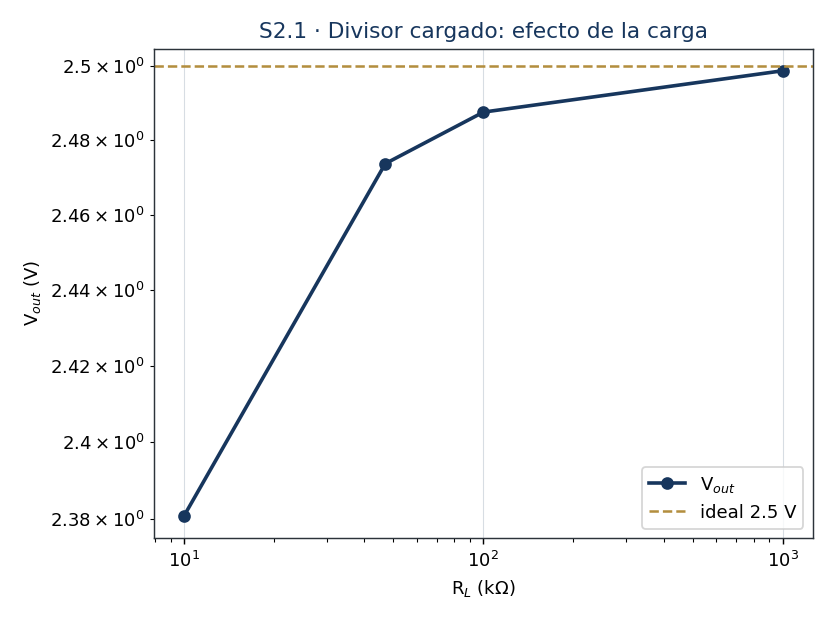
\includegraphics[width=0.78\textwidth]{figs/s21_divisor_cargado.png}
    \end{center}
    \begin{itemize}
      \item El error de carga cae al subir $R_L$; con $R_L\ge 100\,\text{k}\Omega$ queda bajo 1\%.
    \end{itemize}
  \end{frame}

  % ---------------------------------------------------------------------
  \begin{frame}{Errores comunes}
  \begin{table}
    \small
    \begin{tabular}{p{0.34\textwidth}p{0.30\textwidth}p{0.30\textwidth}}
      \toprule
      Error & Consecuencia & Corrección \\
      \midrule
      Usar el divisor en vacío ignorando la carga & Sobreestimar la salida & Paralelar $R_2$ con $R_L$ \\
      No calcular $R_{th}$ para elegir la interfaz & Error de carga por diseño & $R_{in} \ge 100\cdot R_{th}$ \\
      Bajar $R_1$,$R_2$ sin límite & Más consumo/calor & Balancear impedancia vs potencia \\
      Olvidar la impedancia del ADC & Conversión sesgada & Buffer o $R_{in}$ alta \\
      \bottomrule
    \end{tabular}
  \end{table}
\end{frame}

% ---------------------------------------------------------------------
\begin{frame}{Lectura aeroespacial}
  \begin{itemize}
    \item \textbf{Interfaz de sensor:} antes de amplificar se documenta el rango de la señal,
      la tensión de modo común, la $R_{out}$ de cada rama y la impedancia de entrada requerida.
    \item \textbf{ADC de alta impedancia:} los convertidores de alta resolución tienen entrada
      capacitiva; el divisor se carga en el instante de muestreo (sample-and-hold).
    \item \textbf{Consumo presupuestado:} en el EPS, bajar impedancia para reducir error de carga
      aumenta la corriente de reposo; se optimiza contra el presupuesto de potencia.
    \item Un divisor de referencia debe alimentar una carga conocida; si se desconecta, el
      estado queda indefinido (verificador de integridad de cable).
  \end{itemize}
\end{frame}

% ---------------------------------------------------------------------
\begin{frame}{Preguntas de verificación}
  \begin{enumerate}
    \item ¿Por qué la salida cae al conectar una carga a $V_{out}$?
    \item Para error $<1\,\text{\%}$ con $R_{th} = 500\,\Omega$: ¿qué $R_L$ mínima se necesita?
      \uncover<2->{\emph{($\approx \SI{50}{\kilo\ohm}$: $R_L \ge 100\cdot R_{th}$.)}}
    \item ¿Qué conviene más cerca del sensor: $R_1$,$R_2$ altos o bajos? ¿Por qué?
      \uncover<3->{\emph{(Compromiso: impedancia/ruido vs consumo/calor.)}}
    \item Con $R_L = 10\,\text{k}$, ¿qué solución reduce el error: bajar $R_1$,$R_2$ o añadir un buffer?
      \uncover<4->{\emph{(Buffer: $R_{in}$ muy alta $\Rightarrow$ el divisor vuelve a estar en vacío.)}}
    \item Si la salida ideal es 2.5 V y mido 2.38 V, ¿qué información da esa diferencia?
  \end{enumerate}
\end{frame}


\end{document}
